\section{Project Information}\label{sec:project}

\subsection{Project name and introduction}\label{sec:intro}

\textbf{Project name: CarbonPass --- a local-first AI compliance and
energy-optimization copilot for Taiwan's export SMEs.}

CarbonPass is a conversational artificial-intelligence system that converts the
ordinary documents a small factory already holds --- electricity bills,
material invoices, and production records --- into the exact carbon-compliance
artifact its European customers now require, and then schedules the factory's
energy use to cut both cost and emissions. The user experience is a single
sentence: \emph{photograph an electricity bill and invoices inside LINE, answer
three questions in Mandarin or Taiwanese, and receive (a) the verifier-ready
carbon data pack the EU buyer needs, (b) the money that data saves the buyer,
and (c) a production schedule that lowers the power bill and improves next
quarter's emissions.}

\begin{formfield}{Detailed description of AI usage (application form field 2.2)}
CarbonPass is an AI system, not an arithmetic calculator with an interface.
Three distinct AI/ML subsystems carry the product:

\smallskip
\textbf{(1) Document intelligence with allocation reasoning.} A
vision-language model parses heterogeneous, mixed-language, photographed
documents (Taipower bills, Ministry of Finance electronic invoices, handwritten
production logs) into structured activity data. The non-trivial machine-learning
problem is \emph{allocation}: splitting one facility-wide electricity figure
across dozens of product variants and customs (CN) codes, which the EU's
product-level methodology strictly requires but invoices never contain. The
system infers allocation as a constrained-inference problem over production
volumes, machine power ratings, and operating-hour priors, and attaches a
\emph{quantified uncertainty} to every line so a human verifier sees not only a
value but its reliability.

\smallskip
\textbf{(2) A compliance rules engine.} The EU methodology --- simple-versus-complex-goods
logic, precursor (upstream steel) emissions, and the punitive default-value
tables of the 2,400-page implementing regulation\cite{omm} --- is encoded as a
rules engine that populates the European Commission's communication template
and flags each field \emph{actual / default / needs verifier attention}.

\smallskip
\textbf{(3) A carbon- and price-aware scheduler.} Taiwan publishes every
generating unit's output at 10-minute resolution as open
data\cite{taipowerdata}. CarbonPass computes an hourly grid-carbon-intensity
curve from that feed, overlays Taipower time-of-use tariffs\cite{taipower}, and
optimizes when flexible loads (heat-treatment furnaces, compressors, plating
rectifiers) run, subject to order deadlines --- a mixed-integer-programming
baseline refined by a reinforcement-learning policy.

\smallskip
The architecture is \textbf{local-first by design}: parsing and computation run
on the factory's own device or premises, and only the outputs the owner chooses
to send ever leave. This directly answers the trade-secret sensitivity that
otherwise blocks SME adoption of cloud carbon tools.
\end{formfield}

\subsection{Corresponding SDGs}\label{sec:sdg}

\textbf{SDG 8 (Decent Work and Economic Growth)} --- protecting employment and
livelihoods across an export cluster of $\sim$1,800 firms threatened by loss of
EU market access. \textbf{SDG 9 (Industry, Innovation and Infrastructure)} ---
equipping traditional manufacturing SMEs with AI-grade data infrastructure.
\textbf{SDG 12 (Responsible Consumption and Production)} --- product-level
emissions measurement and verified reduction. \textbf{SDG 13 (Climate Action)}
--- extending measurement and mitigation into the SME layer that national
climate targets cannot reach without it.

\subsection{Problem to be resolved and its importance}\label{sec:problem}

\subsubsection*{The target population is specific, named, and economically pivotal}

Taiwan has 1.716 million SMEs (98.87\% of all enterprises), employing 9.19
million people, or 79.3\% of the workforce\cite{moea}. The overwhelming
majority --- shops, services, light logistics --- face no carbon obligation.
This proposal therefore rejects the inflated ``1.7 million SMEs must
decarbonize'' framing and targets the precisely defined population under hard
compulsion today: the \textbf{$\sim$2,600 SMEs} that the Ministry of
Environment (MOENV) identifies as producers of the CBAM-regulated goods Taiwan
exports to the EU\cite{tpt-cbam} (Figure~\ref{fig:funnel}).

\begin{figure}[htbp]
\centering
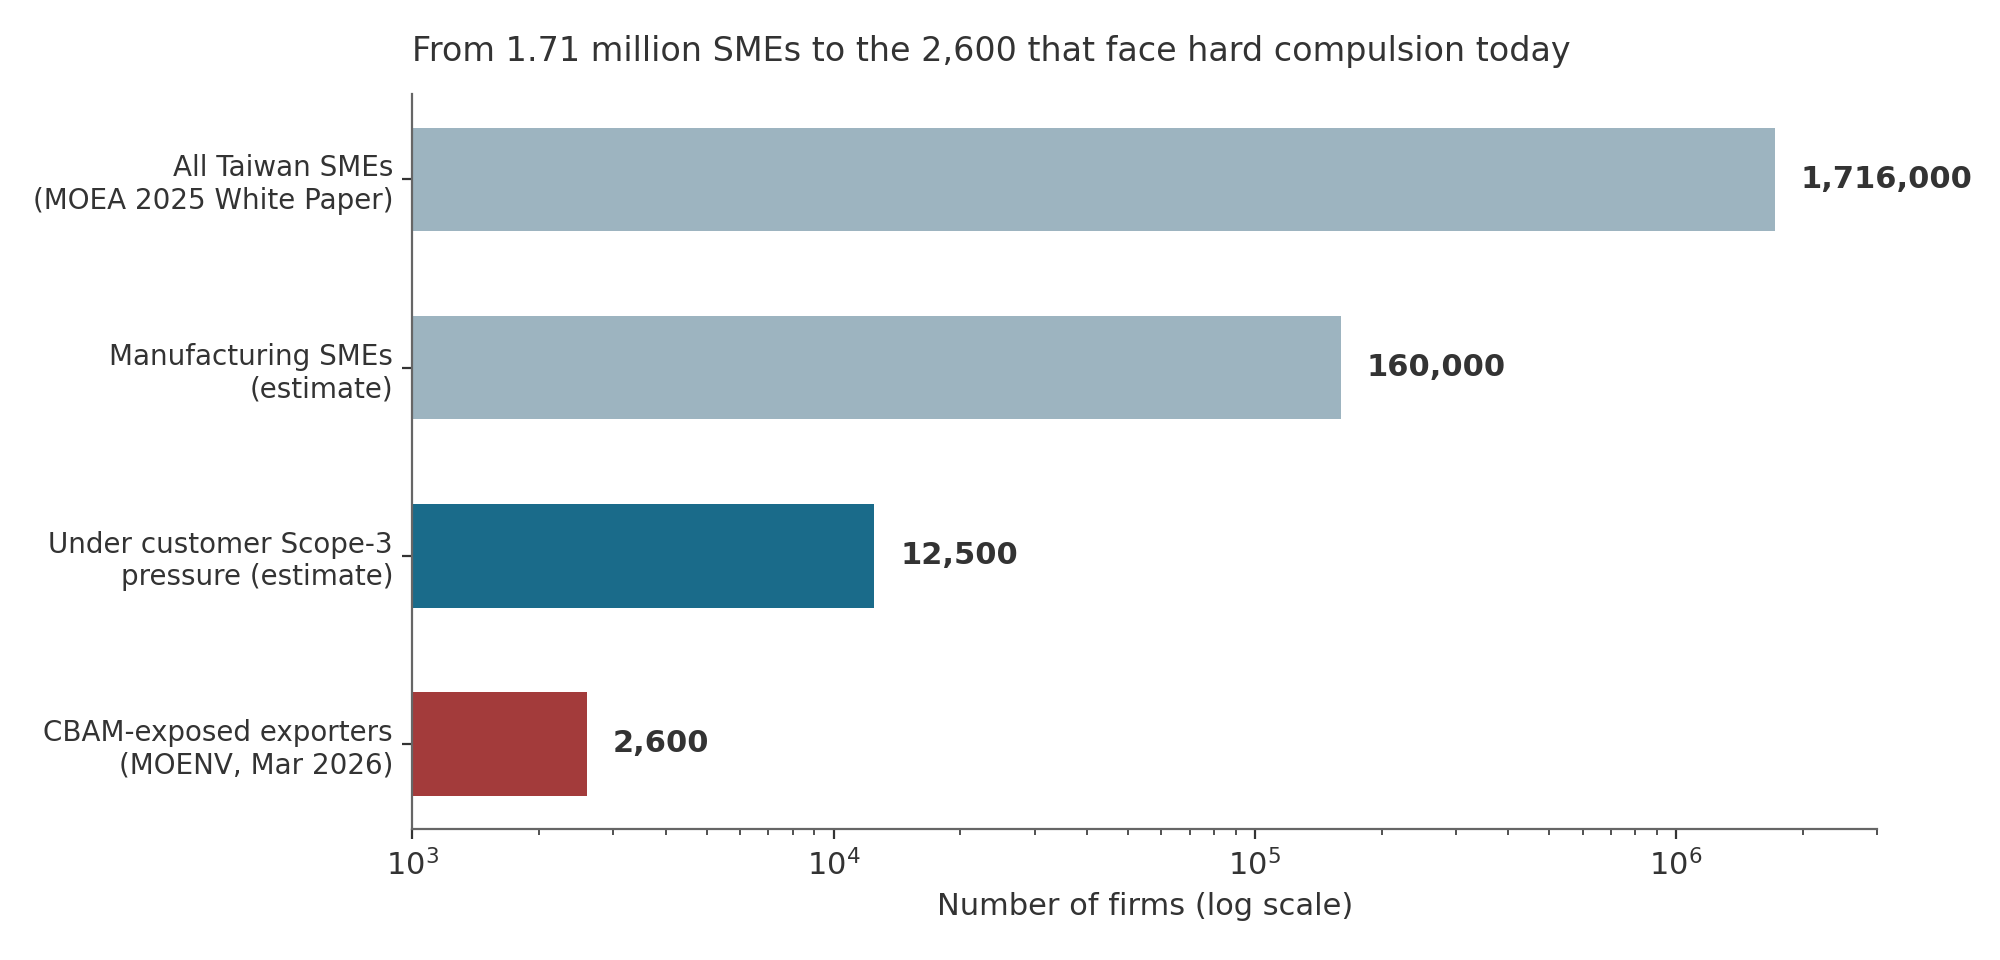
\includegraphics[width=0.9\textwidth]{chart1_funnel.png}
\caption[From 1.716 million SMEs to 2,600 firms under compulsion]{The
addressable population is precisely bounded, not inflated: of Taiwan's 1.716
million SMEs\cite{moea}, the group facing hard compulsion today is the
$\sim$2,600 CBAM-exposed exporters named by MOENV\cite{tpt-cbam}. The two
intermediate bars are this proposal's estimates of the wider,
customer-pressured band.}
\label{fig:funnel}
\end{figure}

These firms are concentrated in one place and one product. The Gangshan--Luzhu
district of Kaohsiung --- the ``Kingdom of Screws'' --- hosts roughly
\textbf{1,800 fastener manufacturers}, about 700 of them organized under the
Taiwan Industrial Fasteners Institute (TIFI)\cite{goebel,ktimes}. Their global
standing is disproportionate to their size (Figure~\ref{fig:sector},
Table~\ref{tab:sector}): a top-three world exporter holding 10--13\% of global
production, shipping $\sim$1.2 million tonnes a year, roughly a quarter of it to
Europe\cite{ktimes,cw}. Nationally, 51.79\% of SMEs are sole proprietorships or
family firms and 58.22\% have operated more than eight years\cite{moea} --- the
demographic profile of the owners now asked to operate EU-grade data systems.

\begin{figure}[htbp]
\centering
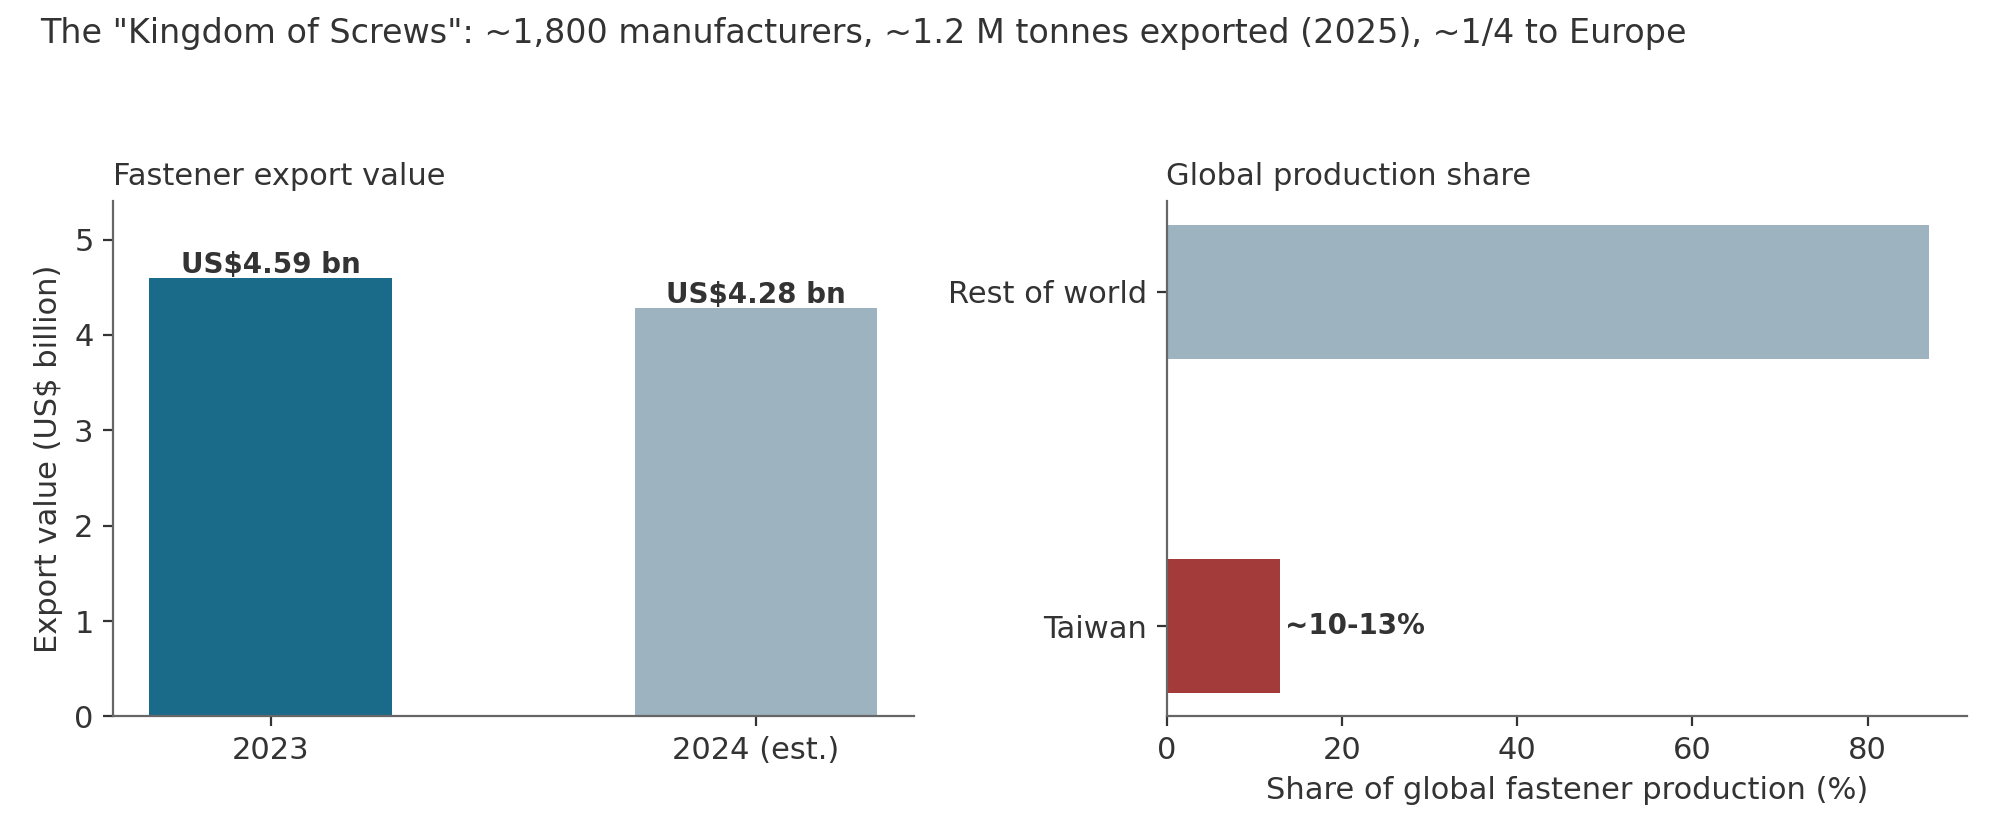
\includegraphics[width=0.9\textwidth]{chart5_sector.png}
\caption[Fastener-sector snapshot]{The beachhead sector: export value (left,
industry statistics\cite{fwexport}) and share of world production
(right\cite{ktimes,goebel}).}
\label{fig:sector}
\end{figure}

\begin{table}[htbp]
\caption{The Taiwanese fastener sector at a glance}
\label{tab:sector}
\small
\begin{tabularx}{\textwidth}{@{}p{0.3\textwidth}Xp{0.2\textwidth}@{}}
\toprule
\textbf{Indicator} & \textbf{Value} & \textbf{Source} \\
\midrule
Global rank & Top-3 exporter (\#2 by value, 2023; \#3 by volume, 2025--26) & CW 2023\cite{cw}; KT 2026\cite{ktimes} \\
Share of world production & $\sim$10--13\% & \cite{ktimes,goebel} \\
Export volume & $\sim$1.2 million tonnes (2025) & \cite{ktimes} \\
Export value & US\$4.59\,bn (2023); $\sim$US\$4.28\,bn (2024, est.) & Fastener World\cite{fwexport} \\
Share destined for Europe & $\sim$one quarter & \cite{cw} \\
Manufacturers & $\sim$1,800 (mostly SMEs; TIFI $\sim$700 members) & \cite{goebel} \\
Embedded emissions & $\sim$2 tCO$_2$e per tonne of product (industry est.) & \cite{specialinsert} \\
\bottomrule
\end{tabularx}
\end{table}

\subsubsection*{The mechanism: how missing data converts into lost orders}

The EU's Carbon Border Adjustment Mechanism (CBAM) entered its definitive,
paying phase on 1 January 2026. Importers of covered steel goods --- including
screws and bolts, customs code CN~7318 --- must buy and surrender CBAM
certificates priced at the official EU rate: \textbf{EUR~75.36 in Q1 and
EUR~75.28 in Q2 2026}\cite{taxud,ecprice,carbonchain}. With verified data, a
tonne of fasteners ($\sim$2 tCO$_2$e embedded\cite{specialinsert}) costs the
buyer about \textbf{EUR~150}. Without it, the importer must use default values
set at the highest observed intensity and marked up 10\% in 2026, 20\% in 2027,
and 30\% from 2028; for complex goods, at least 80\% of reported emissions must
be actual, third-party-verified data\cite{omm,bpc}. Industry analysis puts the
default cost at three to five times the verified cost, reaching
\textbf{30--50\% of product value} on commodity lines\cite{specialinsert}
(Figure~\ref{fig:cbamcost}).

\begin{figure}[htbp]
\centering
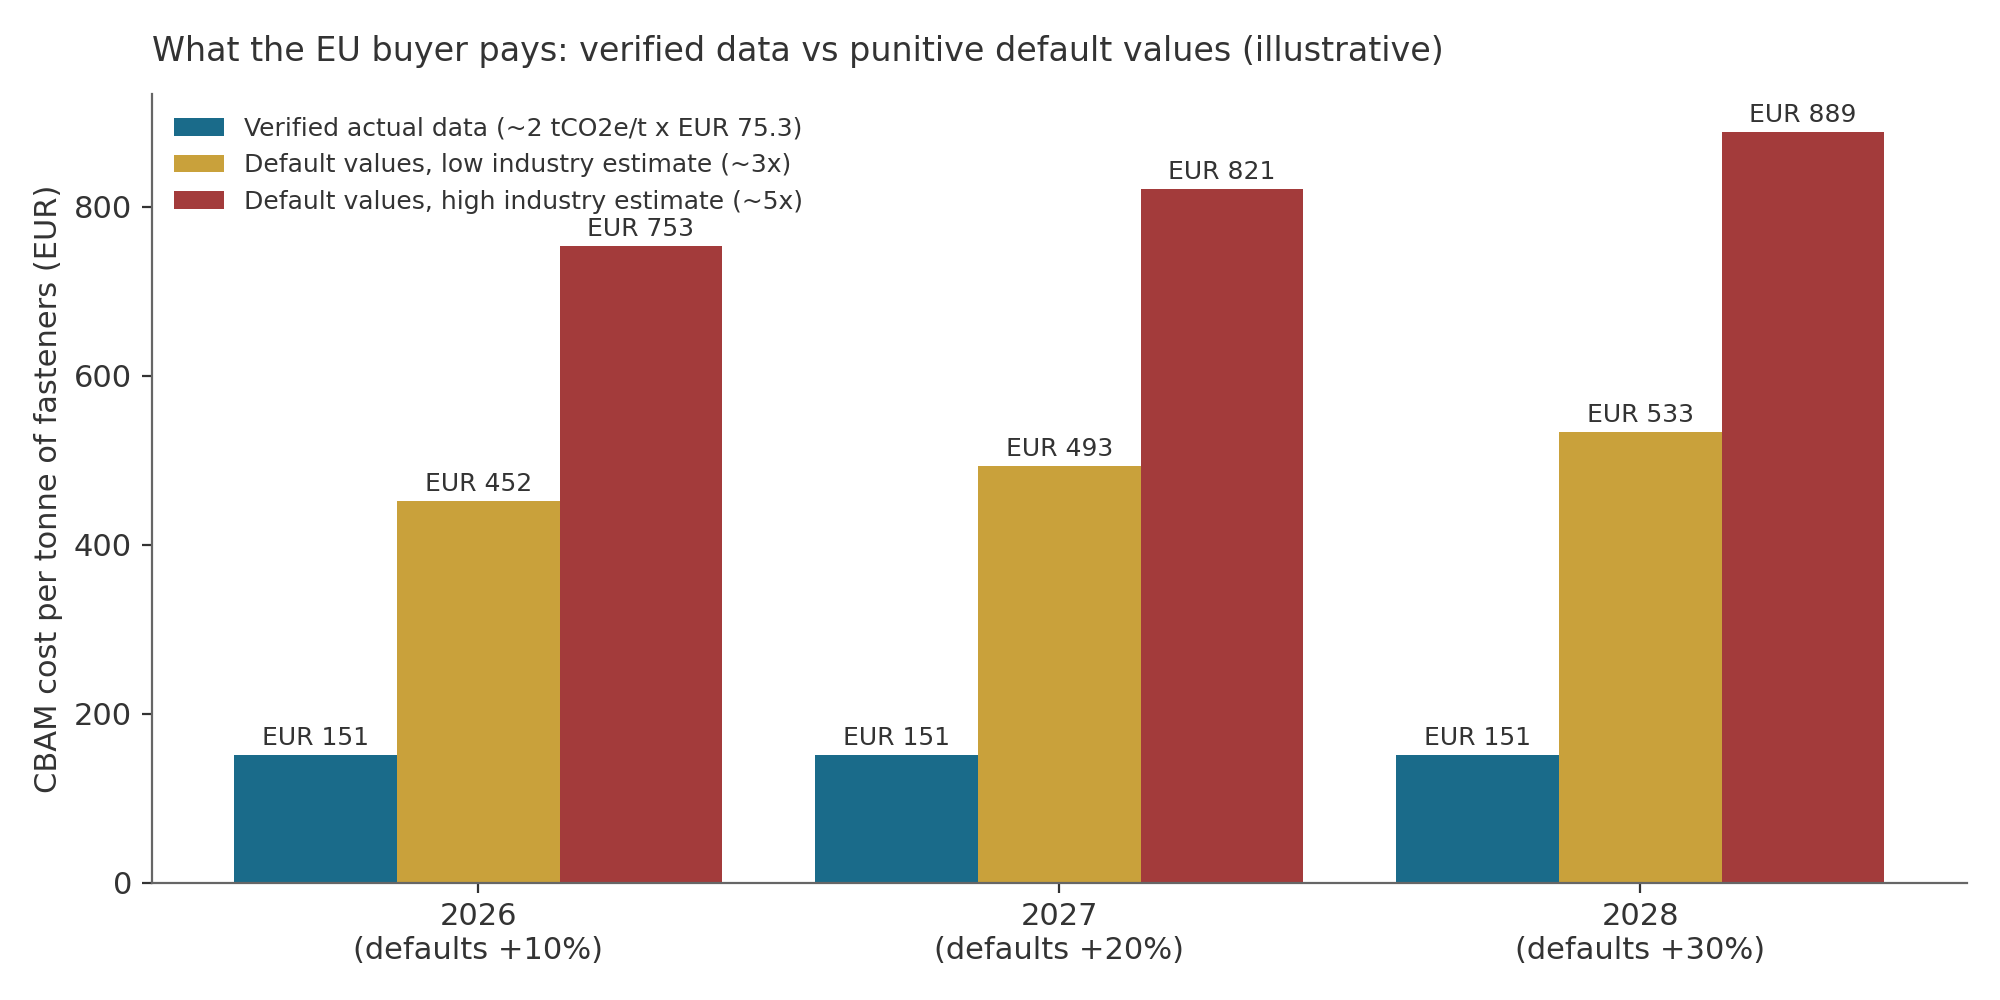
\includegraphics[width=0.9\textwidth]{chart3_cbam.png}
\caption[Verified data versus default values: CBAM cost per tonne]{What the EU
buyer pays per tonne of Taiwanese fasteners: verified actual data versus
punitive defaults, at the official certificate price\cite{ecprice}, escalated
by the regulation's automatic markup schedule\cite{omm}. The difference is the
survival margin of a family factory.}
\label{fig:cbamcost}
\end{figure}

The 50-tonne de minimis exemption does not protect small suppliers: it is
counted cumulatively \emph{per EU importer}, across all of that importer's
suppliers combined. MOENV's Climate Change Administration has warned publicly
that a European distributor buying small lots from several Taiwanese SMEs
crosses the threshold and must then demand verified data from all of
them\cite{tpt-cbam}. The commercial logic is impersonal: an importer facing two
otherwise identical suppliers keeps the one whose data pack arrives with the
shipment. Sector surveys confirm how exposed the cohort is --- \textbf{60\%} of
fast-growing SMEs have completed no carbon inventory, \textbf{80\%} have no
reduction targets, and half cite talent shortage as the binding
constraint\cite{cw}.

\subsubsection*{Why the problem compounds, and why it matters nationally}

The pressure is a rising floor, not a one-time wave. The default markup
escalates automatically to 2028\cite{omm}; the European Parliament votes in
September 2026 on extending CBAM to $\sim$180 further steel and aluminium
product categories from 2028 (Council position adopted June 2026)\cite{akin};
and the EU's Digital Product Passport regime begins phasing in machine-readable
product-sustainability data from 2027\cite{espr}. Domestically, Taiwan's own
carbon price is live: the first fee cycle closed 31 May 2026, collecting
\textbf{NT\$4.97 billion from 461 factories run by 240
companies}\cite{focus,tptfee} (Figure~\ref{fig:fee}), with the 25,000-tonne
threshold set to fall and an emissions-trading pilot approaching
$\sim$2027\cite{ecobiz}. These instruments serve legislated targets: net-zero
by 2050 and the NDC 3.0 commitment of a \textbf{38\%$\pm$2\% cut by
2035}\cite{ndc} (Figure~\ref{fig:ndc}) --- targets that cannot be met by the
$\sim$500 directly regulated large emitters alone, and that require measurement
capillaries reaching into the SME layer this proposal serves.

\begin{figure}[htbp]
\centering
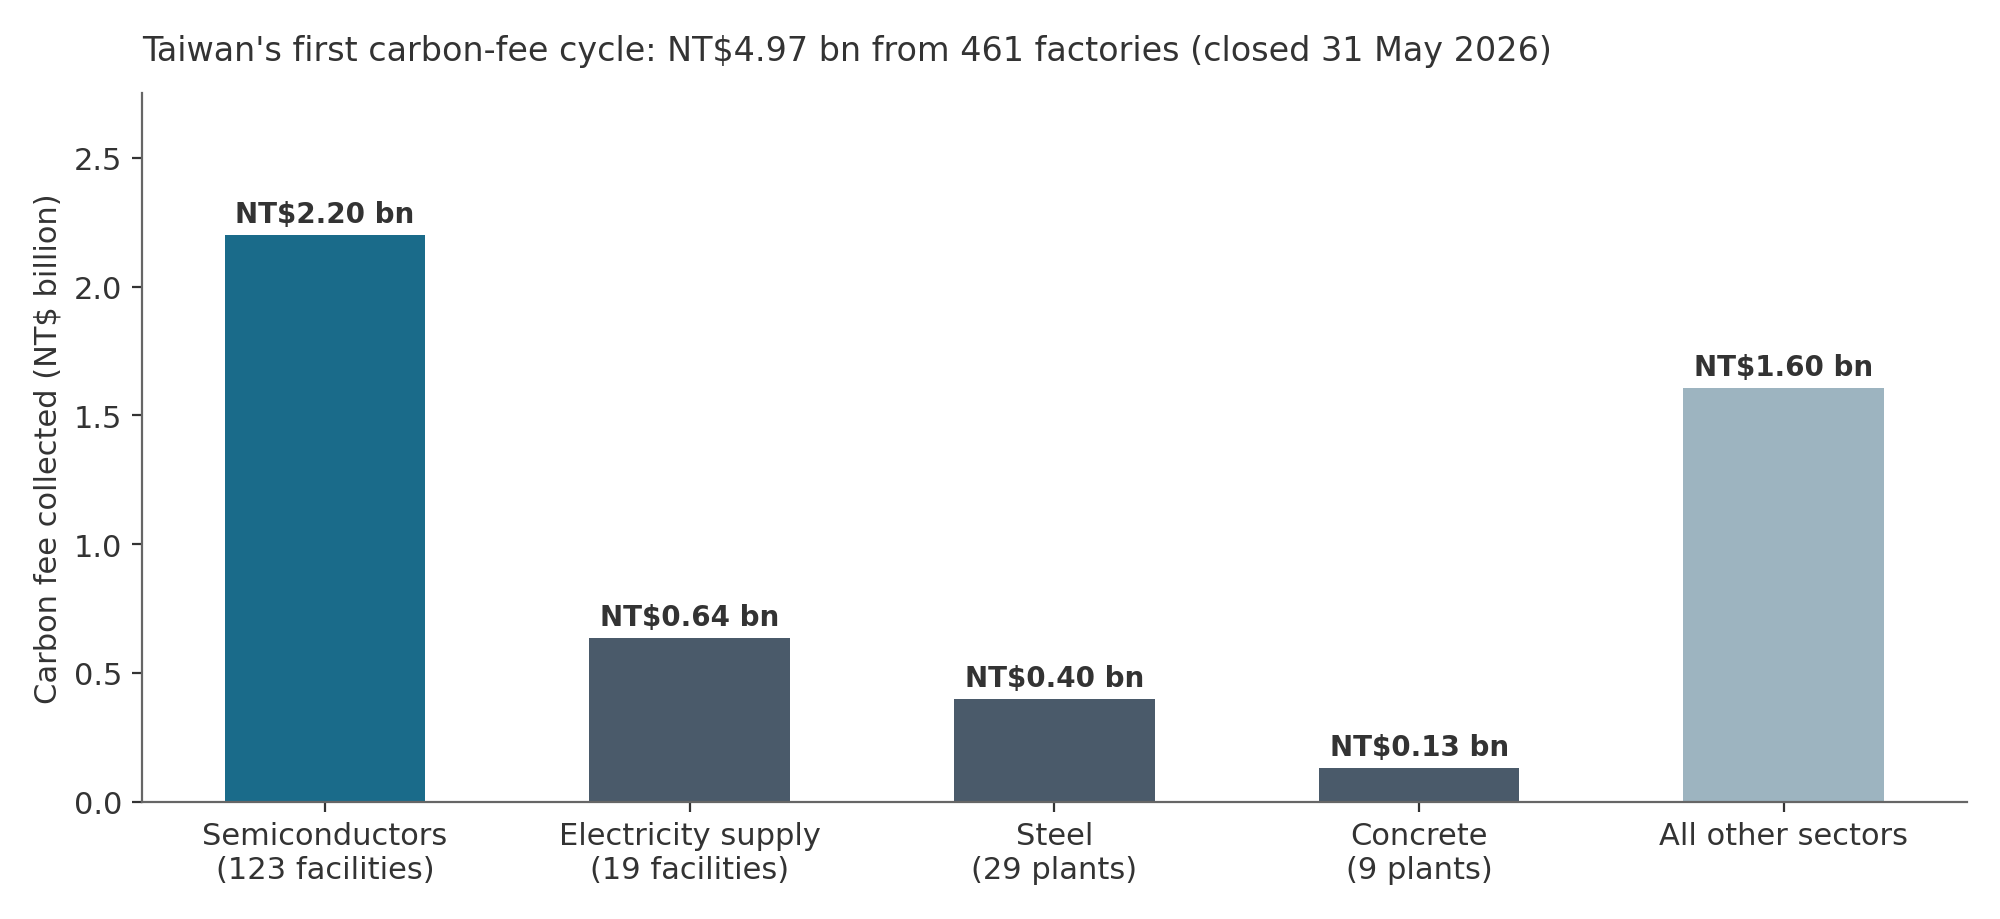
\includegraphics[width=0.86\textwidth]{chart2_fee.png}
\caption[First-cycle carbon-fee revenue by sector]{Taiwan's first carbon-fee
cycle, closed 31 May 2026 (MOENV via Focus Taiwan / Taipei
Times\cite{focus,tptfee}): NT\$4.97 billion, with semiconductors paying 44\%.
The domestic carbon price is live and set to broaden.}
\label{fig:fee}
\end{figure}

\begin{figure}[htbp]
\centering
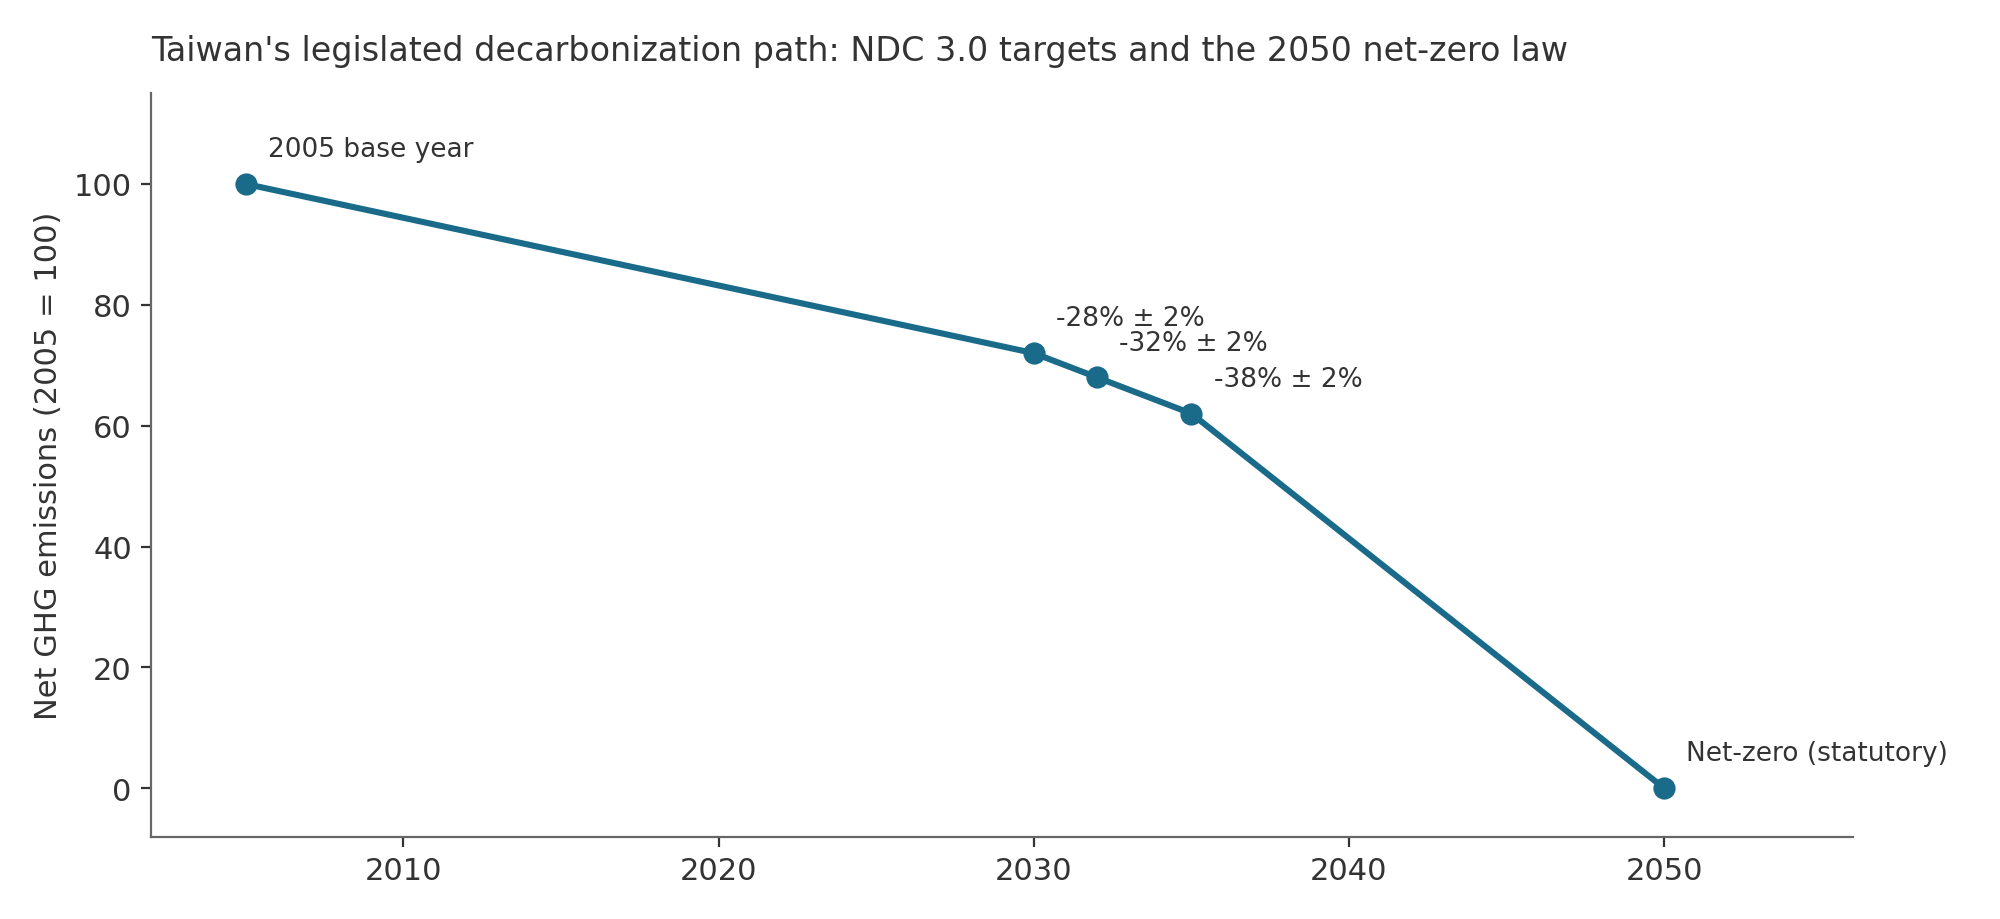
\includegraphics[width=0.86\textwidth]{chart4_ndc.png}
\caption[Taiwan's legislated decarbonization path]{Taiwan's legislated
emissions path: the NDC 3.0 targets (MOENV, 2025\cite{ndc}) and the statutory
2050 net-zero goal. Reaching them requires extending measurement into the SME
base.}
\label{fig:ndc}
\end{figure}

\subsection{Related stakeholders and their roles}\label{sec:stakeholders}

The \textbf{target audience is the fastener SME owner} --- chosen because this
group carries live legal-commercial compulsion, has the lowest digital
readiness, and is geographically and industrially concentrated enough for a
focused pilot to generalize. The remaining stakeholders form the adoption and
verification chain around that user.

\begin{table}[htbp]
\caption{Stakeholders, roles, and benefits (target audience highlighted)}
\label{tab:stakeholders}
\small
\begin{tabularx}{\textwidth}{@{}p{0.29\textwidth}X@{}}
\toprule
\textbf{Stakeholder} & \textbf{Role and benefit} \\
\midrule
\textbf{Fastener SME owners \emph{(target audience)}} & Primary users: retain EU customers, cut power costs, and gain a standing carbon capability in their own language \\
EU importers and their declarants & Receive template-ready supplier data; avoid punitive default costs\cite{omm} \\
TIFI ($\sim$700 members) and MIRDC & Pilot recruitment, domain validation, and the channel for cluster-scale rollout\cite{goebel} \\
MOENV / Climate Change Administration & Their CBAM help platform\cite{tpt-cbam} gains the computation layer it currently lacks; SME carbon-fee readiness rises \\
MOEA / SMESA & The CAAS education stack\cite{caas} gains an execution tool for SME competitiveness \\
Taiwan Power Company & Its open data and AMI infrastructure\cite{taipower,taipowerdata} become directly value-generating for small industry \\
Accredited verifiers & Receive structured, uncertainty-annotated files rather than raw paper --- faster, cheaper verification \\
Banks (green finance) & Verified SME carbon data for sustainability-linked lending \\
\bottomrule
\end{tabularx}
\end{table}

\subsection{Description of solution functions}\label{sec:solution}

\subsubsection*{How the target audience uses it}

Mr.~Lin, a 61-year-old owner in Gangshan, opens LINE. The assistant greets him
in Taiwanese and asks for a photo of last month's Taipower bill. He photographs
it, then the steel wire-rod invoices, and answers three plain questions about
production. Within about ninety seconds he receives: a \textbf{carbon data
pack} for his screws, per customs code, in the European Commission's template
and flagged line-by-line for the verifier; a \textbf{one-screen argument} he
can forward to his buyer --- \emph{your cost with my data: $\approx$EUR~150/t;
without it: EUR~450--750/t and rising}; and a \textbf{scheduling suggestion} ---
shift the heat-treatment furnace to the 02:00--06:00 window this month, for an
estimated saving in NT\$ on the bill and in kilograms of CO$_2$, both of which
flow into next quarter's pack automatically. No web portal, no consultant, and
no data leaving his building.

\subsubsection*{How the problem is solved, stage by stage}

\begin{table}[htbp]
\caption{The CarbonPass pipeline: from shoebox documents to market access}
\label{tab:pipeline}
\small
\begin{tabularx}{\textwidth}{@{}p{0.22\textwidth}X@{}}
\toprule
\textbf{Stage} & \textbf{What happens} \\
\midrule
Inputs the SME already has & Taipower bills, material invoices, production records --- photographed in LINE, in Mandarin/Taiwanese \\
Document intelligence + allocation & Vision-language parsing of messy, mixed-format documents; facility energy allocated across product lines and CN codes with quantified uncertainty \\
Compliance rules engine & EU methodology (simple/complex goods, precursors, default tables\cite{omm}) encoded into field-level guidance and the Commission's template \\
Grid-aware scheduler & Hourly grid carbon intensity from Taipower's open 10-minute feed\cite{taipowerdata} + time-of-use tariffs\cite{taipower} $\to$ MILP + reinforcement-learning shift plans \\
Outputs & CBAM data pack per CN code; organizational inventory (by-product); buyer-cost delta screen; monitored before/after reduction ledger \\
\bottomrule
\end{tabularx}
\end{table}

The two modules reinforce each other. The Data-Pack Engine (Module~1) answers
the immediate compliance demand; the Grid-Aware Scheduler (Module~2) then
lowers real consumption, and every avoided tonne shrinks the next data pack.
The reduction ledger is structured to the baseline-and-monitoring logic of
ISO~14064-2 --- structured to the standard's logic, with certification
remaining the accredited verifier's act. The conversational LINE interface
(Module~3) is not cosmetic: it is the mechanism by which an analog-native owner
participates at all, and is therefore the operative form of digital inclusion
in this project.

\subsection{Differences from existing solutions}\label{sec:diff}

Taiwan's current ecosystem is an \emph{awareness} stack; CarbonPass is the
missing \emph{execution} layer. The audit below was verified instrument by
instrument in July 2026.

\begin{table}[htbp]
\caption{Capability audit: what exists, and what none of it does}
\label{tab:gap}
\small
\begin{tabularx}{\textwidth}{@{}p{0.25\textwidth}p{0.33\textwidth}X@{}}
\toprule
\textbf{Instrument} & \textbf{What it does} & \textbf{What it does not do} \\
\midrule
CAAS ``SME Carbon Reduction Service Station'' (MOEA)\cite{caas} & Courses, articles, consultant referrals & No computation; not a reporting tool \\
IDB Carbon Emissions Calculator (MOEA)\cite{idb} & Rough annual company-level CO$_2$e from bills & No product-level allocation, no CN codes, no CBAM format \\
MOENV CBAM Help Platform (Mar 2026)\cite{tpt-cbam} & Information and consultation & Explicitly informational; computes nothing \\
Taipower app / eBill\cite{taipower} & Consumption charts, tariff simulation & No emissions conversion; no compliance artifacts \\
tre100 pledge platform (CIER)\cite{tre100} & Renewable-energy commitments registry & No measurement tooling \\
Consultants / ESG software\cite{chanchin} & Real one-off ISO certificates & Per-engagement pricing; cannot serve recurring per-product demand across 2,600 firms \\
\bottomrule
\end{tabularx}
\end{table}

\textbf{The difference in one sentence:} CarbonPass is the only tool that
converts SME-native documents into importer-ready, verifier-structured,
per-CN-code emissions data --- repeatably, in the owner's own language, at
near-zero marginal cost --- and it is designed to \emph{integrate} with the
government's existing platforms rather than compete with them.

\subsection{Expected benefits (quantified)}\label{sec:benefits}

\begin{table}[htbp]
\caption{Expected benefits, with basis of estimate}
\label{tab:benefits}
\small
\begin{tabularx}{\textwidth}{@{}p{0.32\textwidth}Xp{0.2\textwidth}@{}}
\toprule
\textbf{Benefit} & \textbf{Quantification} & \textbf{Basis} \\
\midrule
CBAM cost avoided per tonne & $\approx$EUR~300--600/t (verified $\approx$150 vs.\ defaults 450--750, rising with markups) & Official price\cite{ecprice}; industry multiples\cite{specialinsert} \\
Compliance labor per data pack & Hours instead of consultant-weeks; recurring at near-zero marginal cost & Cluster ISO precedents priced per engagement\cite{chanchin} \\
Energy cost reduction via load shifting & Peak/off-peak tariff spread of several$\times$ on shiftable loads (est.\ 5--15\% of bill for furnace-heavy plants; measured in pilot) & Taipower TOU schedules\cite{taipower} \\
Emissions reduction & Measured on-meter, logged to ledger; each avoided tonne also cuts the buyer's certificate cost & Grid EF 0.474 kgCO$_2$e/kWh\cite{moeaea} \\
Population served at beachhead & 2,600 CBAM-exposed SMEs within a $\sim$1,800-firm, top-3 world export cluster & MOENV\cite{tpt-cbam}; \cite{goebel,ktimes} \\
National alignment & Extends measurement into the SME layer, supporting NDC 3.0 ($-$38\%$\pm$2\% by 2035) & \cite{ndc} \\
\bottomrule
\end{tabularx}
\end{table}
